\documentclass[12pt, a4paper, reqno]{amsart}

\usepackage{amsfonts}
\usepackage{amsmath}
\usepackage{anysize}
\usepackage{graphicx}
\usepackage[hidelinks]{hyperref}
\hypersetup{
    colorlinks=true,
    linktoc=all,
    allcolors=black,
    final
}

\marginsize{1in}{1in}{1in}{1in}

\begin{document}

\begin{titlepage}
	\centering
    {\scshape\LARGE John Wiley \& Sons, Inc.\par}
	\vspace{1cm}
	{\huge\bfseries Advanced Engineering Mathematics\par}
	\vspace{2cm}
	{\scshape\Large 10th Edition\par}
	\vspace{1.5cm}
	{\Large\itshape Erwin Kreyszig\par}
	\vfill
	In collaboration with\par
    ~Herbert \textsc{Kreyszig}\par
    ~Edward ~J. \textsc{Norton}

	\vfill

% Bottom of the page
	{\large \today\par}
\end{titlepage}

\renewcommand{\abstractname}{3 Line Abstract}

\section*{Abstract}
\textit{The model of the vibrating string will consist of a PDE 
(“wave equation”) and 
additional conditions. To obtain the PDE, we consider the forces acting on a 
small portion of the string (Fig. 286). This method is typical of modeling in 
mechanics and elsewhere.}

\tableofcontents

\section{Introduction}

We continue our work from Sec. 12.2, where we modeled a vibrating string and obtained
the one-dimensional wave equation. We now have to complete the model by adding
additional conditions and then solving the resulting model.
The model of a vibrating elastic string (a violin string, for instance)
consists of a onedimensional wave equation.

\section{Results}

\begin{equation}
    \frac{\partial^2{u}}{\partial{t^2}} = c^2\frac{\partial^2{u} \\
    }{\partial{x^2}} \qquad \qquad c^2 = \frac{T}{\rho}
\end{equation}

\begin{equation}
    \frac{ \partial^2{u} }{ \partial{t^2} } = F\ddot{G} \qquad \text{and} \\
    \qquad \frac{ \partial^2{u} }{ \partial{x^2} } = F''G
\end{equation}

\begin{equation}
    u_n(x,t)=(B_n\cos{\lambda_n t} + B_n^\star\sin{\lambda_n t}) \\
    \sin{\frac{n\pi}{L} x} \quad \quad (n=1,2,\dotsb).
\end{equation}

\begin{equation}                                                                
    \sin{\frac{n\pi x}{L}}=0 \qquad \text{at} \\                             
    \qquad x=\frac{L}{n}, \frac{2L}{n},\dotsb,\frac{n-1}{n}L,                      
\end{equation}  

\begin{equation}                                                                
    F=Ae^{\mu x} = Be^{-\mu x}                                                  
\end{equation}   

\section{Conclusion}

\begin{center}
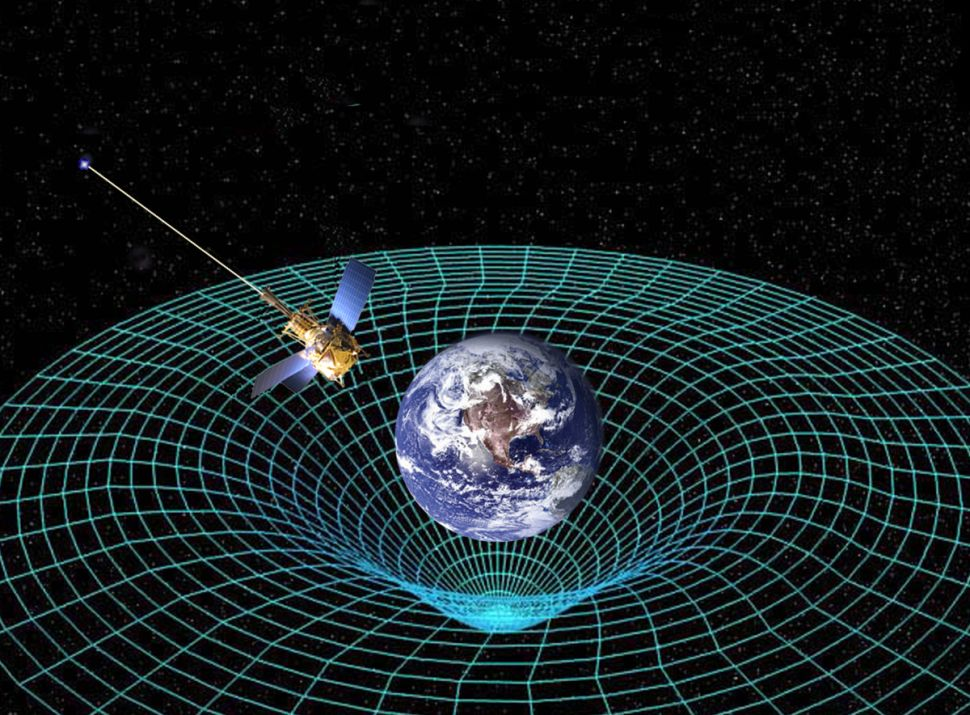
\includegraphics[height=5cm]{../time-1.jpg}

Here is some text that I want to have in between the pictures.

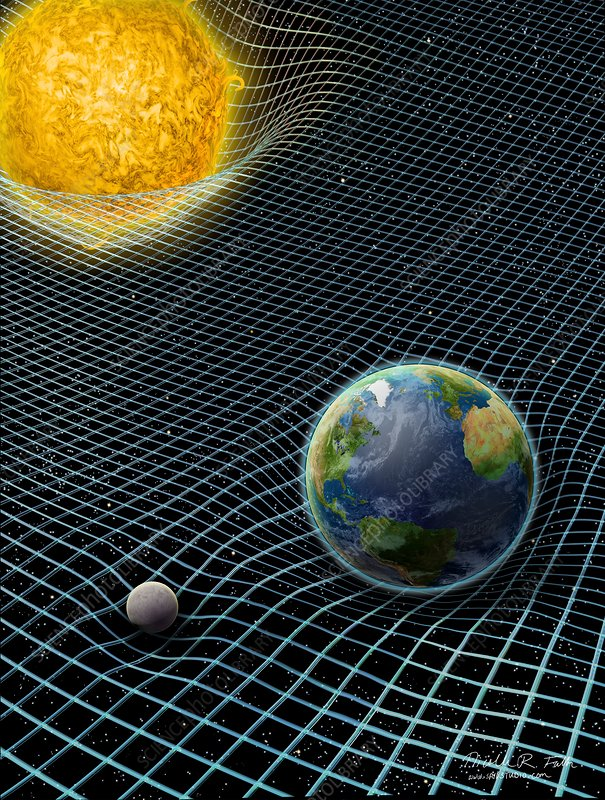
\includegraphics[height=5cm]{../time-2.jpg}
\end{center}

\section{Acknowledgements}

We are indebted to former teachers, colleagues, and students who helped us 
directly or indirectly in preparing this book, in particular this new edition. 
We profited greatly from discussions with engineers, physicists, 
mathematicians, computer scientists, and others, and from their written 
comments.

\section{References}

\begin{enumerate}
    \item \LaTeX book, Wikibooks. Retrieved from: https://en.wikibooks.org/wiki/LaTeX
    \item Overleaf \LaTeX Documentation. Retrieved from: \newline
        https://www.overleaf.com/learn/latex/Main\_Page
\end{enumerate}
\begin{itemize}
    \item Advances in Applied Mathematics. 1981. Hal Schenck, Catherine Yan
    \item Differential Equations. Springer
\end{itemize}

\end{document}
